\documentclass[a4paper]{article}

\usepackage[czech]{babel} %https://github.com/michal-h21/biblatex-iso690
\usepackage[
   backend=biber      % if we want unicode 
  ,style=iso-numeric % or iso-numeric for numeric citation method          
  ,babel=other        % to support multiple languages in bibliography
  ,sortlocale=cs_CZ   % locale of main language, it is for sorting
  ,bibencoding=UTF8   % this is necessary only if bibliography file is in different encoding than main document
]{biblatex}

\usepackage[utf8]{inputenc}
\usepackage{fancyhdr}
\usepackage{amsmath}
\usepackage{amssymb}
\usepackage[left=2cm,right=2cm,top=2.5cm,bottom=2.5cm]{geometry}
\usepackage{graphicx}
\usepackage{pdfpages}
\usepackage{url}

\usepackage{siunitx}
\sisetup{locale = DE, separate-uncertainty = true    } %kdybych chtel +/-

\usepackage{float}
\newfloat{graph}{htbp}{grp}
\floatname{graph}{Graf}
\newfloat{tabulka}{htbp}{tbl}
\floatname{tabulka}{Tabulka}

\renewcommand{\thefootnote}{\roman{footnote}}

\pagestyle{fancy}
\lhead{Praktikum III - (7) Ověření Fresnelových vzorců}
\rhead{Vladislav Wohlrath}
\author{Vladislav Wohlrath}

\bibliography{source}


\begin{document}

\begin{titlepage}
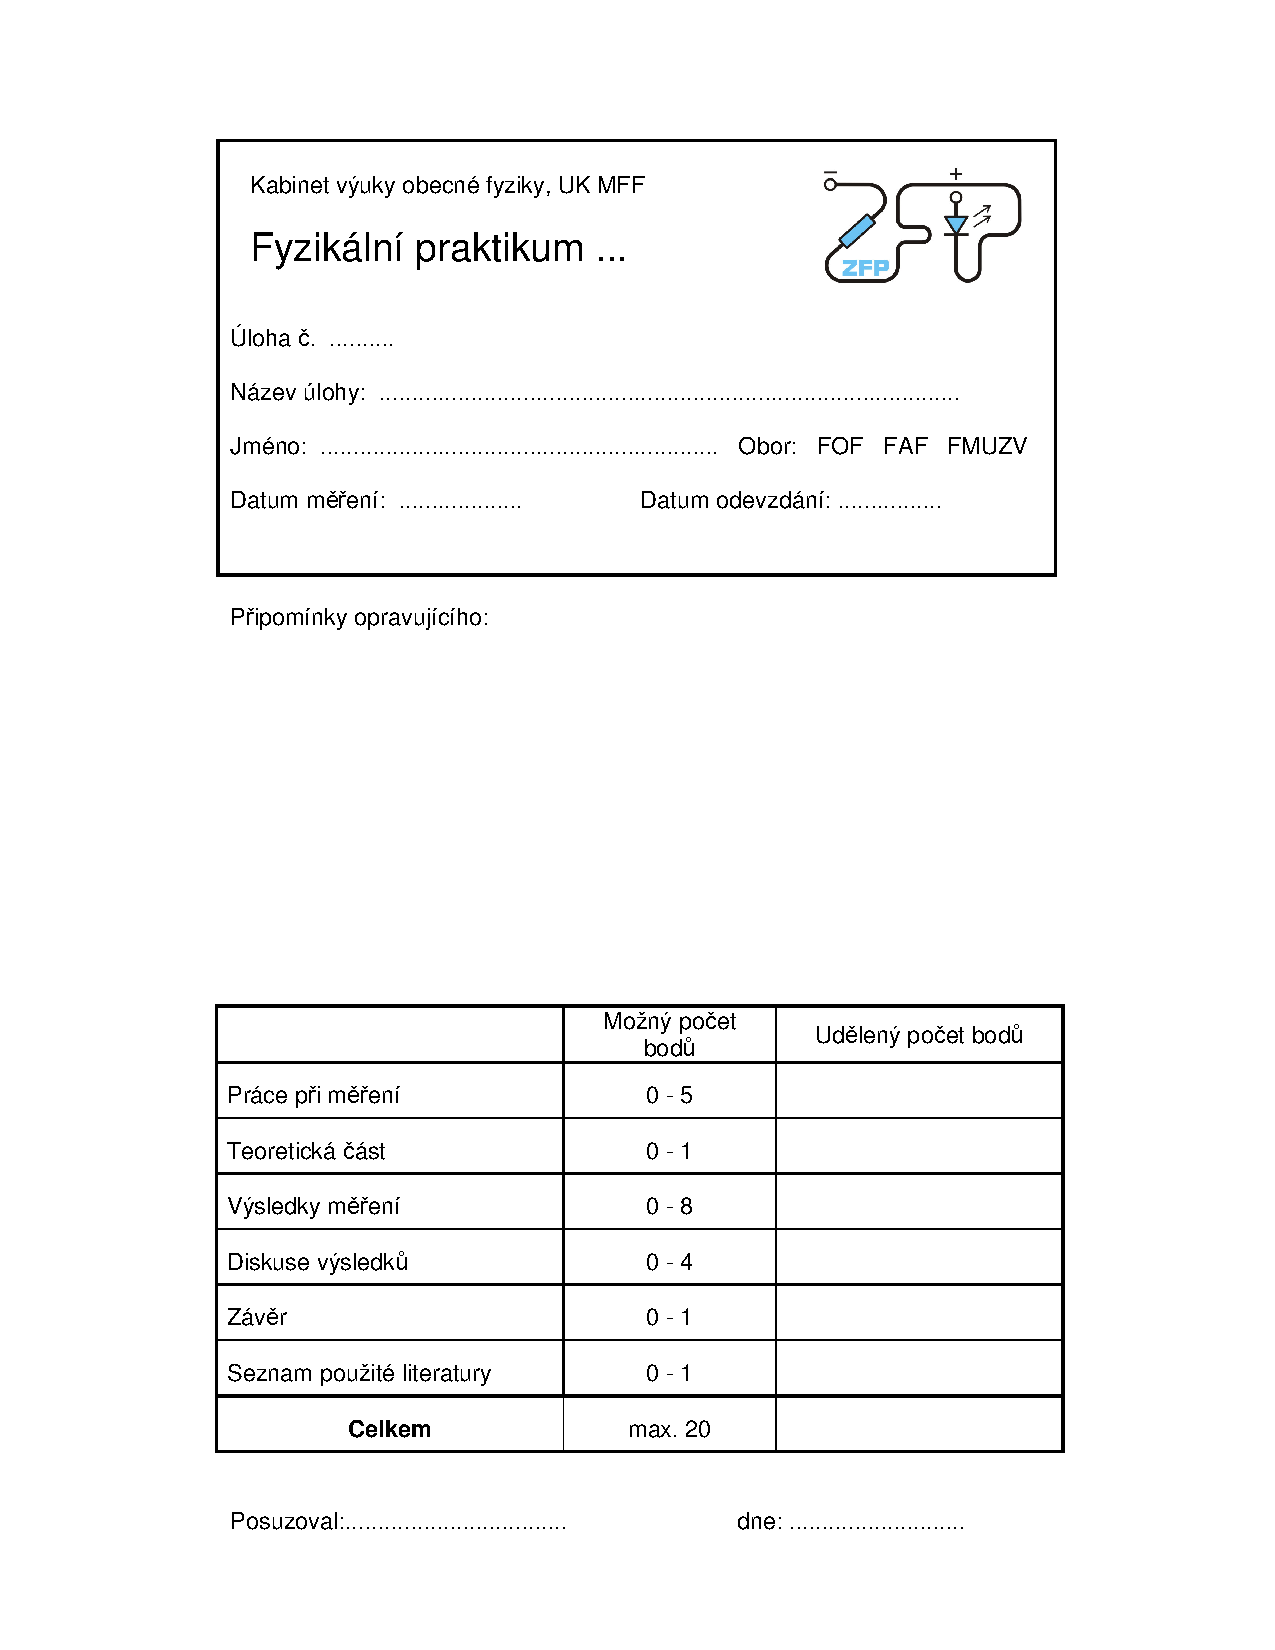
\includepdf[pages={1}]{./graficos/tit.pdf}
\end{titlepage}

\section*{Pracovní úkoly}
\begin{enumerate}
\item Najděte směr snadného průchodu polarizátoru užívaného v aparatuře.
\item Ověřte, že zdroj světla je polarizován kolmo k vodorovné rovině.
\item Na přiložených vzorcích proměřte závislost intenzity odraženého světla na úhlu dopadu pro \emph{TE} i \emph{TM} polarizaci.
\item Naměřené výsledky porovnejte s teoretickým průběhem závislostí.
\item Určete indexy lomů měřených vzorků a jejich relativní chybu.

\end{enumerate}

%Teoretická část
\section*{Teoretická část}

%Výsledky měření
\section*{Výsledky měření}

%Diskuze výsledků
\section*{Diskuze}

%Závěr
\section*{Závěr}


\printbibliography[title={Seznam použité literatury}]

\end{document}